%!TEX root =Graphulo_MatrixMultiply_HPEC2015.tex

\section{Discussion}
\label{sDiscussion}

\subsection{Related Work} %Analogy to MapReduce with Accumulo Scanners, Iterators and BatchWriters:
%\todo[inline]{Cannon's algorithm, other SpGEMM}
Bulu\c{c} and Gilbert studied message passing algorithms for SpGEMM
such as Sparse SUMMA, most of which use 2D block decompositions \cite{buluc2012parallel}.
Unfortunately, 2D decompositions are difficult in Accumulo 
and message passing even more so.
In this work, we use Accumulo's native 1D decomposition along rows 
and do not rely on tablet server communication
apart from shuffling partial products of $\matr{C}$ via BatchWriters.


Our outer product method could have been implemented in MapReduce %x\cite{dean2008mapreduce} 
on Hadoop or its successor YARN \cite{vavilapalli2013apache}.
There is a natural analogy from TableMult to MapReduce:
the map phase scans rows from $\matr{A^\tr}$ and $\matr{B}$
and generates a list of partial products from TwoTableIterator;
the shuffle phase sends partial products to correct tablets of $\matr{C}$ via BatchWriters;
the reduce phase sums partial products using Combiners.
Examining the conditions on which MapReduce 
reading from and writing to Accumulo's RFiles directly
can outperform Accumulo-only solutions
is worthy future work.

%TableMult Design Alternatives
%% A common Accumulo pattern is to %run multiple clients %that scan disjoint and continuous table sections in parallel.
%% scan and write from multiple clients in parallel.
%% %In fact, 
%% The high insert rates of \cite{kepner2014achieving}
%% were obtained using 
%% parallel clients aware of tablet locations.
%% %% Kepner et al used parallel clients and tablet location info
%% %% to insert at record-setting rates \cite{kepner2014achieving}.

A common Accumulo pattern is to 
scan and write from multiple clients in parallel;
in fact, researchers obtained 
considerably high insert rates using parallel client strategies \cite{kepner2014achieving}.
We chose to build Graphulo as a service within Accumulo
instead of assuming a multiple client capability,
such that Graphulo is as accessible as possible to diverse client environments.

The strategy in \cite{kepner2014achieving} 
also used %information on tablet assginment to tablet servers
%physical 
tablet location information
to determine where clients could write locally.
Knowing tablet-to-tablet-server assignment could likewise aid Graphulo, 
not only to minimize network traffic
but also
 to partly eliminate Apache Thrift RPC serialization,
which prior work has shown is a bottleneck for scans % writes?
when iterator processing is light \cite{sawyer2013understanding}.
%Enhancing Accumulo for non-Thrift, local access may 
Such an enhancement would access a local tablet server by method call 
in place of Scanners and BatchWriters.
%use a new access inter-process chanel 
%optimized for 

%% %% In order to make Graphulo as accessible to client environments %configurations
%% %% as possible, we built Graphulo as a service within Accumulo 
%% %% instead of assuming multiple client capabilities.
%% %%% We avoid the multiple client pattern because it increases client software complexity,
%% %%% whereas we aim for a service within Accumulo that works for any client.
%% As described in \cite{sawyer2013understanding}, 
%% table scans that do not perform significant iterator processing
%% bottleneck on communication overhead at the client due to Apache Thrift serialization.
%% %% %filtering or other server-side computation 
%% %% Future work may eliminate this bottleneck by 
%% %% avoiding 
%% % avoid RPCs
%% % local tablet location information
%% %We gain a chance to eliminate Thrift overhead %by moving computation to the server,
%% Future work may eliminate Thrift overhead
%% for scans and writes to tablets located on the same tablet server.
%% %though the current version does not do so because standard Scanners and BatchWriters serialize as clients would.

\subsection{Design Alternative: Inner-Outer Product Hybrid}

%bridge inner and outer product
It is worth reconsidering the inner product method from our initial design
because it has an opposite performance profile as 
Figure~\ref{fInnerOuterSpectrum}'s left and right depict: 
inner product bottlenecks on scanning whereas outer product bottlenecks on writing.
At the expense of multiple passes over input matrices, inner product emits 
partial products in order and immediately pre-summable,
%more efficiently in that emitted entries are in order and partial products can sum immediately, 
reducing the number of entries written to Accumulo to the minimum possible.
Outer product reads inputs in a single pass
but emits entries out of order and has little chance to pre-sum, 
instead writing individual partial products to $\matr{C}$.
Table~\ref{tResultsParams} quantifies that outer product writes
2.5 to 3 times more entries than inner product for power law inputs.
In the worst case, multiplying a fully dense $N \times M$ with an $M \times L$ matrix,
outer product emits $M$ times more entries than inner product.



%LRU cache enables the bridge
Is it possible to blend inner and outer product SpGEMM methods,
choosing a middle point in Figure~\ref{fInnerOuterSpectrum}
with equal read and write bottlenecks for overall greater performance?
In the following generalization, 
partition parameter $P$ varies behavior between
inner product at $P=N$ and outer product at $P=1$:

\removelatexerror
\begin{algorithm}[H]
\vspace{\algspace}
\SetKwBlock{fore}{for}{} 
\SetKw{emit}{emit}
\fore($p = 1\col P$){
\fore($k = 1\col M$){
\fore({$i = \left( \floor*{\dfrac{(p-1)N}{P}}+1 \right) \col \floor*{\dfrac{p N}{P}}$}){
\fore($j = 1\col L$){
%\vspace{4pt}
{$\matr{C}(i,j) \mathrel{\oplus}= \matr{A}(i,k) \otimes \matr{B}(k,j)$}
}}}}
\vspace{\algspace}
\end{algorithm}

The hybrid algorithm runs $P$ passes through $\matr{B}$,
each of which has write locality to a vertical partition of $\matr{C}$ of size $N/P \times L$.
Pre-summing ability likewise varies inversely with $P$, 
though actual pre-summing depends on
$\matr{A}$ and $\matr{B}$'s  sparsity distribution
as well as how many positions of $\matr{C}$ the TableMult iterators cache.
Figure~\ref{fInnerOuterSpectrum}'s center depicts the $P=2$ case.

\begin{figure}[t]
%\vspace{-4pt}
\centering
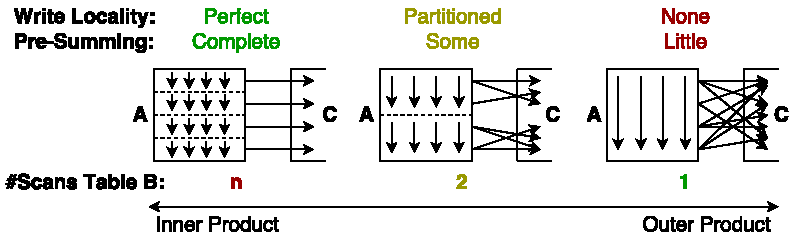
\includegraphics[width=\linewidth]{InnerOuterSpectrum}
%\vspace{-14pt}
\caption{Tradeoffs between Inner and Outer Product}
\label{fInnerOuterSpectrum}
%\vspace{-4pt}
\end{figure}


A challenge for any hybrid algorithm is mapping it to Accumulo infrastructure.
We chose outer product because it more naturally fits Accumulo, 
using iterators for one-pass streaming computation, 
BatchWriters to handle unsorted entry emission and Combiners to defer summation.
The above hybrid algorithm resembles 2D block decompositions,
and so maximizing its performance may be challenging 
given limited data layout control and unknown data distribution.
%Further investigation is future work.
%Hybrid solutions might consider locality groups or transpose tables to enable column-oriented scanning
%and the distribution of tablets to tablet server cost modeling to 
%% We may realize greater performance by considering data placement among tablet servers, 
%% but such a consideration would require accessing and perhaps manipulating
%% Accumulo's internal state and non-public API.
%% We suggest this paper's approach as a balance between top performance and implementation stability.


Nevertheless, possible design criteria are to select a small $P$ to minimize passes through $\matr{B}$,
while also choosing $P$ large enough so that $\ceil{NL/P}$ entries fit in memory
(dense matrix worst case), which guarantees complete pre-summing.
The latter criterion may be relaxed with decreasing matrix density.


\subsection{TableMult in Algorithms}
%% Several optimization opportunities exist for TableMult as a primitive in larger algorithms.
%% Suppose we have a program $\matr{C} = \matr{A B}; \matr{D} = \matr{CC}; \matr{A} \mathrel{\oplus}= \matr{D}$.
%% We would save two round trips to disk if we could mark $\matr{C}$ and $\matr{D}$ as 
%% ``temporary tables,'' i.e. tables intermediate to an algorithm that should be held in memory 
%% and not written to Hadoop if possible.
%% Combiners in TableMult do enable one optimization:
%% summing $\matr{CC}$ into $\matr{A}$ directly by rewriting the program as 
%% $\matr{C} = \matr{AB}; \matr{A} \mathrel{\oplus}= \matr{CC}$.

Several optimization opportunities exist for TableMult as a primitive in larger algorithms.
Given row $\matr{A}$ of starting vertices and graph adjacency matrix $\matr{B}$, 
suppose we wish to union the vertices reached in two steps from those in $\matr{A}$ 
into $\matr{A}$ via the program
 $\matr{C} = \matr{AB}; \matr{D} = \matr{CB}; \matr{A} \mathrel{\oplus}= \matr{D}$,
as one way of calculating $\matr{A} \mathrel{\oplus}= \matr{AB}^2$ via TableMult calls.
Such calculations are useful for finding vertices reachable in an even number of steps.
We would save two round trips to disk if we could mark $\matr{C}$ and $\matr{D}$ as 
``temporary tables,'' i.e. tables intermediate to an algorithm that should be held in memory 
and not written to Hadoop if possible.
Combiners in TableMult do enable one optimization:
summing $\matr{CB}$ into $\matr{A}$ directly by rewriting the program as 
$\matr{C} = \matr{AB}; \matr{A} \mathrel{\oplus}= \matr{CB}$.

A \emph{pipelining} optimization streams entries from a TableMult 
to computations taking its result as input. 
Outer product pipelining is difficult
because it cannot guarantee writing every partial product for a particular element 
 to $\matr{C}$ until it finishes,
whereas inner product's complete pre-summing emits elements ready for use downstream.
More ambitiously, \emph{loop fusion} merges iterator stacks 
for successive computations into one. 

Optimizing computation on NoSQL databases is challenging in the general case because
NoSQL databases typically avoid query planner features 
customary of SQL databases in exchange for raw performance.
% and simplicity of implementation
NewSQL databases aim in part to achieve the best of both worlds---performance and query planning \cite{grolinger2013data}.
We aspire to make a small step for Accumulo in the direction of NewSQL with current Graphulo research.






\section{Conclusions}
\label{sConclusions}

In this work we showcase the design of TableMult, a Graphulo server-side implementation of the 
SpGEMM GraphBLAS matrix math kernel in the Accumulo database.
We compare inner and outer product approaches and show how outer product 
better fits Accumulo's iterator model.  The implementation shows excellent single node performance, 
achieving write rates near 400,000 per second, 
which is consistent with the single node peak write rate for Accumulo \cite{kepner2014achieving}.
Performance experiments show good scaling for scaled problem sizes and suggest good scaling for fixed size problems,
but these require additonal experiments on a larger cluster to confirm.

In addition to topics from Section~\ref{sDiscussion}'s discussion, 
future research efforts include
implementing the remaining GraphBLAS kernels, 
developing graph algorithms that use the Graphulo library
and delivering to the Accumulo community.
